%!Mode:: "TeX:UTF-8"

\section{UML类图}
UML的类图关系分为: 关联、聚合/组合、依赖、泛化(继承)。而其中关联又分为双向关联、单向关联、自身关联。

关系所表现的强弱程度依次为:组合>聚合>关联>依赖。

\subsection{关联}


双向关联:
C1-C2:指双方都知道对方的存在,都可以调用对方的公共属性和方法。

在GOF的设计模式书上是这样描述的:虽然在分析阶段这种关系是适用的,但我们觉得它对于描述设计模式内的类关系来说显得太抽象了,因为在设计阶段关联关系必须被映射为对象引用或指针。对象引用本身就是有向的,更适合表达我们所讨论的那种关系。所以这种关系在设计的时候比较少用到,关联一般都是有向的。

双向关联在代码的表现为双方都拥有对方的一个指针,当然也可以是引用或者是值。

% \begin{figure}[ht]
  % \begin{center}
    % 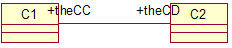
\includegraphics[keepaspectratio,width=0.36\paperwidth]{Pictures/UML/UMLdoubleAssoc.JPG}
    % \caption{双向关联}
    % \label{fig:doubleAssoc}
  % \end{center}
% \end{figure}

% 单向关联:
% C3->C4:表示相识关系,指C3知道C4,C3可以调用C4的公共属性和方法。没有生命期的依赖。一般是表示为一种引用。

% \begin{figure}[ht]
  % \begin{center}
    % 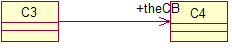
\includegraphics[keepaspectratio,width=0.36\paperwidth]{Pictures/UML/UMLuniAssoc.JPG}
    % \caption{单向关联}
    % \label{fig:uniAssoc}
  % \end{center}
% \end{figure}

% \subsection{组合/聚合}
% 当类之间有整体-部分关系的时候,我们就可以使用组合或者聚合。二者在代码上未必有区别,区别存在于语义上。

% 聚合:表示C9聚合C10,但是C10可以离开C9而独立存在。

% \begin{figure}[ht]
  % \begin{center}
    % 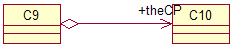
\includegraphics[keepaspectratio,width=0.36\paperwidth]{Pictures/UML/UMLAggregation.JPG}
    % \caption{聚合}
    % \label{fig:Aggregation}
  % \end{center}
% \end{figure}


% \begin{figure}[ht]
  % \begin{center}
    % 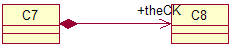
\includegraphics[keepaspectratio,width=0.36\paperwidth]{Pictures/UML/UMLComposition.JPG}
    % 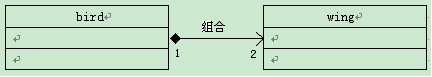
\includegraphics[keepaspectratio,width=0.36\paperwidth]{Pictures/UML/UmlCompositionNumbered.png}
    % \caption{组合}
    % \label{fig:UMLComposition}
  % \end{center}
% \end{figure}
% 组合(也有人称为包容、合成):一般是实心菱形加实线箭头表示,如上图所示,表示的是C8被C7包容,而且C8不能离开C7而独立存在。但这是视问题域而定的,例如在关心汽车的领域里,轮胎是一定要组合在汽车类中的,因为它离开了汽车就没有意义了。但是在卖轮胎的店铺业务里,就算轮胎离开了汽车,它也是有意义的,这就可以用聚合了。在《敏捷开发》中还说到,A组合B,则A需要知道B的生存周期,即可能A负责生成或者释放B,或者A通过某种途径知道B的生成和释放。



% 合成(Composition)是一种强的“拥有”关系,体现了严格的部分和整体的关系,部分和整体的生命周期一样。
% 合成关系用实心菱形加实线箭头表示。数字1、2是基数,表明这一端的类可以有几个实例。n表示可能有无数个实例。关联和聚合也可以有基数。

% \subsection{依赖}

% 指C5可能要用到C6的一些方法,也可以这样说,要完成C5里的所有功能,一定要有C6的方法协助才行。C5依赖于C6的定义,一般是在C5类的头文件中包含了C6的头文件。注意,要避免双向依赖。一般来说,不应该存在双向依赖。

% 在形式上一般是A中的某个方法把B的对象作为参数使用(假设A依赖于B)。如下:
% \begin{verbatim}
% #include "B.h"
% class A
% ...{
          % void Func(B &b);
% }
% \end{verbatim}


% \begin{figure}[ht]
  % \begin{center}
    % 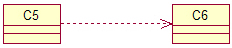
\includegraphics[keepaspectratio,width=0.36\paperwidth]{Pictures/UML/UMLDependancy.JPG}
    % \caption{依赖}
    % \label{fig:UMLDependancy}
  % \end{center}
% \end{figure}

% 那依赖和聚合/组合、关联等有什么不同呢?

% 关联是类之间的一种关系,例如老师教学生,老公和老婆,水壶装水等就是一种关系。这种关系是非常明显的,在问题领域中通过分析直接就能得出。

% 依赖是一种弱关联,只要一个类用到另一个类,但是和另一个类的关系不是太明显的时候(可以说是“uses”了那个类),就可以把这种关系看成是依赖,依赖也可说是一种偶然的关系,而不是必然的关系,就是“我在某个方法中偶然用到了它,但在现实中我和它并没多大关系”。例如我和锤子,我和锤子本来是没关系的,但在有一次要钉钉子的时候,我用到了它,这就是一种依赖,依赖锤子完成钉钉子这件事情。
% 组合是一种整体-部分的关系,在问题域中这种关系很明显,直接分析就可以得出的。例如轮胎是车的一部分,树叶是树的一部分,手脚是身体的一部分这种的关系,非常明显的整体-部分关系。

% 上述的几种关系(关联、聚合/组合、依赖)在代码中可能以指针、引用、值等的方式在另一个类中出现,不拘于形式,但在逻辑上他们就有以上的区别。

% 这里还要说明一下,所谓的这些关系只是在某个问题域才有效,离开了这个问题域,可能这些关系就不成立了,例如可能在某个问题域中,我是一个木匠,需要拿着锤子去干活,可能整个问题的描述就是我拿着锤子怎么钉桌子,钉椅子,钉柜子;既然整个问题就是描述这个,我和锤子就不仅是偶然的依赖关系了,我和锤子的关系变得非常的紧密,可能就上升为组合关系(让我突然想起武侠小说的剑不离身,剑亡人亡...)。这个例子可能有点荒谬,但也是为了说明一个道理,就是关系和类一样,它们都是在一个问题领域中才成立的,离开了这个问题域,他们可能就不复存在了。


% \subsection{泛化}
% 泛化(Generalization)表示一个更泛化的元素和一个更具体的元素之间的关系。泛化是用于对继承进行建模的UML元素。在Java中,用extends关键字来直接表示这种关系。

% \begin{figure}[ht]
  % \begin{center}
    % 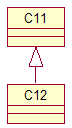
\includegraphics[keepaspectratio,width=0.05\paperwidth]{Pictures/UML/UMLinheri.JPG}
    % \caption{泛化(OOP中“继承”同泛化方向相反)}
    % \label{fig:UMLinheri}
  % \end{center}
% \end{figure}

% \subsection{实现(Realization)}
% OOP中的接口继承用实现(Realization)关系进行建模。
% 实现关系指定两个实体之间的一个合同。换言之,一个实体定义一个合同,而另一个实体保证履行该合同。
% 对Java应用程序进行建模时,实现关系可直接用implements关键字来表示。

% \begin{figure}[ht]
% \centering
	% \begin{minipage}[t]{0.4\textwidth}  
	 % 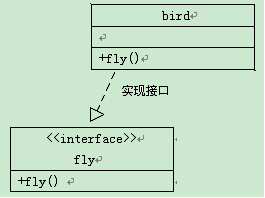
\includegraphics[keepaspectratio,width=0.2\paperwidth]{Pictures/UML/UmlInterfaceRec.png}
    % \caption{接口继承矩形表示法}
    % \label{fig:UMLInterfaceInheri}
	% \end{minipage}
	% \begin{minipage}[t]{0.4\textwidth} 
   % 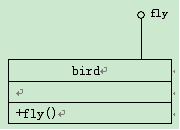
\includegraphics[keepaspectratio,width=0.2\paperwidth]{Pictures/UML/UmlInterfaceCandy.png}
    % \caption{接口继承棒棒糖表示法}
    % \label{fig:UMLInterfaceInheri}
	% \end{minipage} 
% \end{figure}



\clearpage





